\section{Auswertung}
\label{sec:Auswertung}
\subsection{Bestimmung der Halbwertsbreite und Intensität}
DIe Intensitätsverteilung des Röntgenstrahls kann durch eine Gaußfunktion der Form
\begin{equation}
    I(\theta)=\frac{I_0}{\sqrt{2\cdot \pi \cdot \sigma^2}} \cdot \exp\left(-\frac{(\theta-\mu)^2}{2\cdot \sigma^2}\right)+b
\end{equation}
beschrieben werden. Dabei ist $I_0$ die maximale Intensität, $\mu$ der Mittelwert, $\sigma$ die Standardabweichung und $b$ der Untergrund. Die Halbwertsbreite $\Delta \theta$ ist definiert als der Abstand von $\theta$ zu den Punkten, an denen die Intensität auf die Hälfte des Maximums abgefallen ist. Die Halbwertsbreite kann durch die Formel
\begin{equation}
    FWHM = 2\cdot \sqrt{2\cdot \ln(2)}\cdot \sigma
\end{equation}
berechnet werden. Die Daten sind mit Hilfe von Curve-Fit aus der Python Bibliothek Sci-py mit einer Gaussfunktion gefittet worden.
Die Messwerte und der Fit sind in Abbildung \ref{fig:Detectorscan} dargestellt. Die Fitparameter betragen
\begin{align*}
    I_0 &= \SI{3.42(0.04)e5}{\per\second}, \\
    \mu &= \SI{0.0031(0.0005)}{\degree}, \\
    \sigma &= \SI{0.0372(0.0004)}{\degree}, \\
    b &= \SI{5.2(0.9)e4}{\per\second}.
\end{align*}
Damit ist die maximale Intensität $I_0=\SI{3.42(0.04)e5}{\per\second}$ und die Halbwertsbreite $FWHM = \SI{0.087(0.001)}{\degree}$.
\begin{figure}[H]
    \centering
    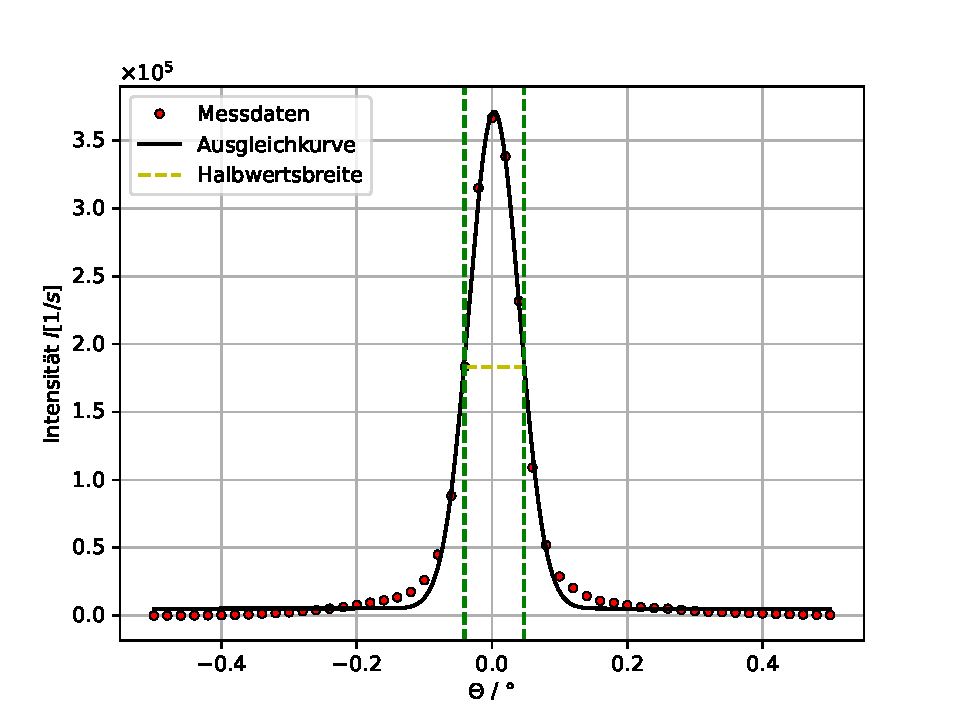
\includegraphics[width=0.8\textwidth]{plots/Detectorscan.pdf}
    \caption{Winkelabhängigkeit der Intensität des Röntgenstrahls}
    \label{fig:Detectorscan}
\end{figure}
\subsection{Bestimmung des Geometriewinkels}
In Abbildung \ref{fig:Zscan} ist der Z-Scan dargestellt. Aus der Breite des Abfalls der gemessenen Intensität, sobald die Probe getroffen wird, kann 
der Strahldurchmesser bestimmt werden. Als Grenzen sind der erste Messpunkt vor dem linearen Abfall und der erste Messpunkt nach dem linearen Abfall gewählt worden.
genommen worden. Daraus ergibt sich ein Strahldurchmesser von $d=\SI{0.16}{\milli\meter}$.
\begin{figure}[H]
    \centering
    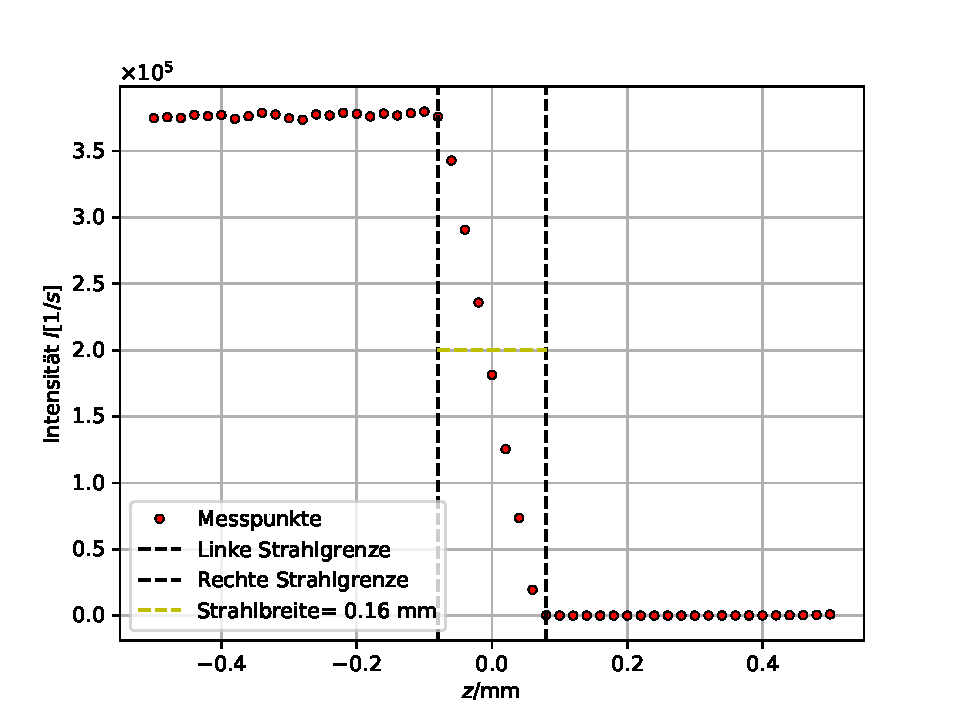
\includegraphics[width=0.8\textwidth]{plots/Zscan.pdf}
    \caption{Z-Scan zur Bestimmung der Strahlbreite}
    \label{fig:Zscan}
\end{figure}
In Abbildung \ref{fig:Xscan} ist der X-Scan dargestellt. An dem Ort an dem sich die Probe befindet fällt die Intensität ab. Daher kann aus der Breite des Abfalls ide Probenbreite 
bestimmt werden. Dafür sind jeweils drei Messpunkte des Randes für eine lineare Ausgleichsgerade $y=a\cdot x+b$ genommen worden. Die Probenbreite wurde bei der halben Intensität gemessen.
Durch Umstellen der Gleichung für die Ausgleichsgerade ergibt sich dann die Position der Ränder. 
Die Parameter der linearen Ausgleichsgerade für die Ränder, welcher mit der Numpy-Funktion Polyfit erstellt worden ist, betragen
\begin{align*}
    a_1 &= \SI{-9e5}{\per\milli\meter\second}, \\
    b_1 &= \SI{-8.5e6}{\milli\meter\second}, \\
    a_2 &= \SI{7.7e5}{\per\milli\meter\second}, \\
    b_2 &= \SI{-5e6}{\milli\meter\second}.
\end{align*}
Damit ergibt sich die Probenbreite zu $d=\SI{22.44}{\milli\meter}$.
\begin{figure}[H]
    \centering
    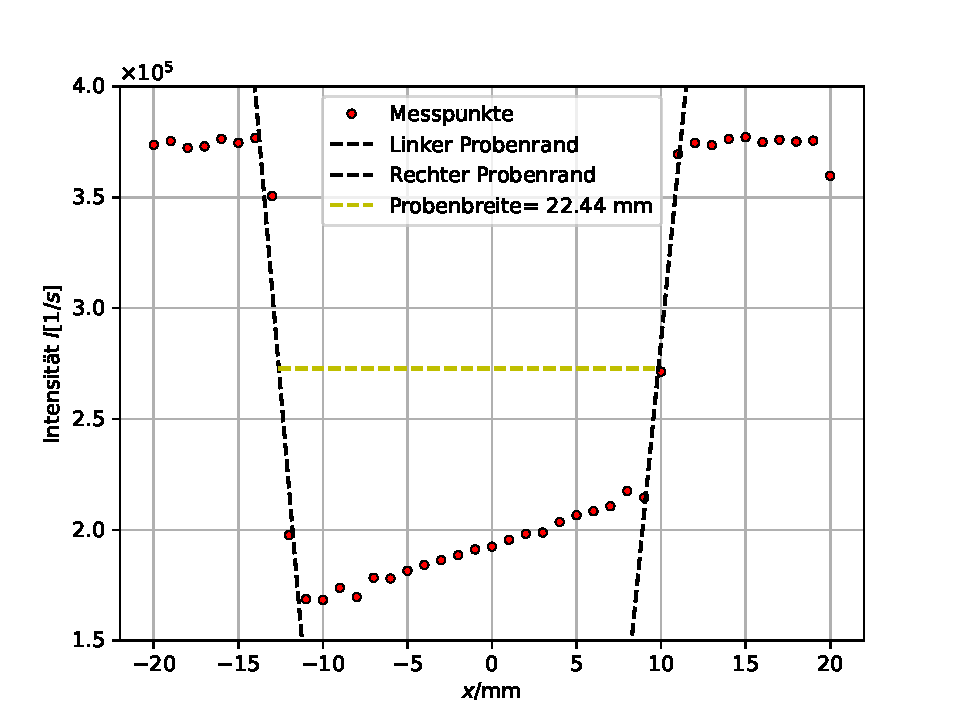
\includegraphics[width=0.8\textwidth]{plots/Xscan.pdf}
    \caption{X-Scan zur Bestimmung der Probenbreite}
    \label{fig:Xscan}
\end{figure}

\begin{figure}[H]
    \centering
    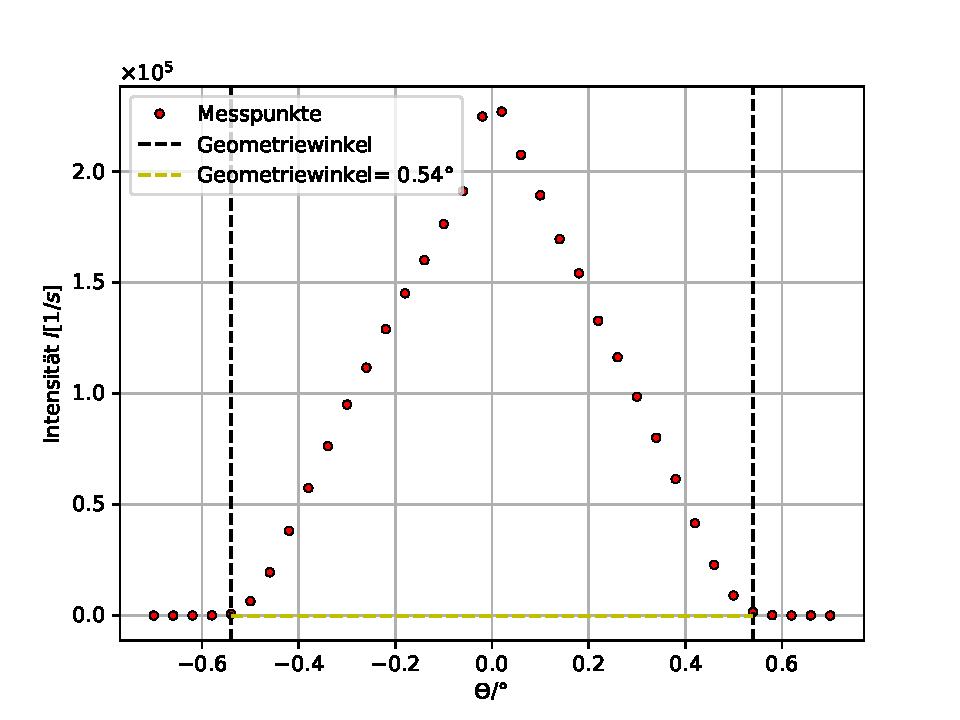
\includegraphics[width=0.8\textwidth]{plots/Rocking.pdf}
    \caption{Rockingscan zur Bestimmung des Geometriewinkels}
    \label{fig:Rocking}
\end{figure}
\subsection{Bestimmung der Rauigkeit und des Brechungsindex von Grenzschichten}
\begin{figure}[H]
    \centering
    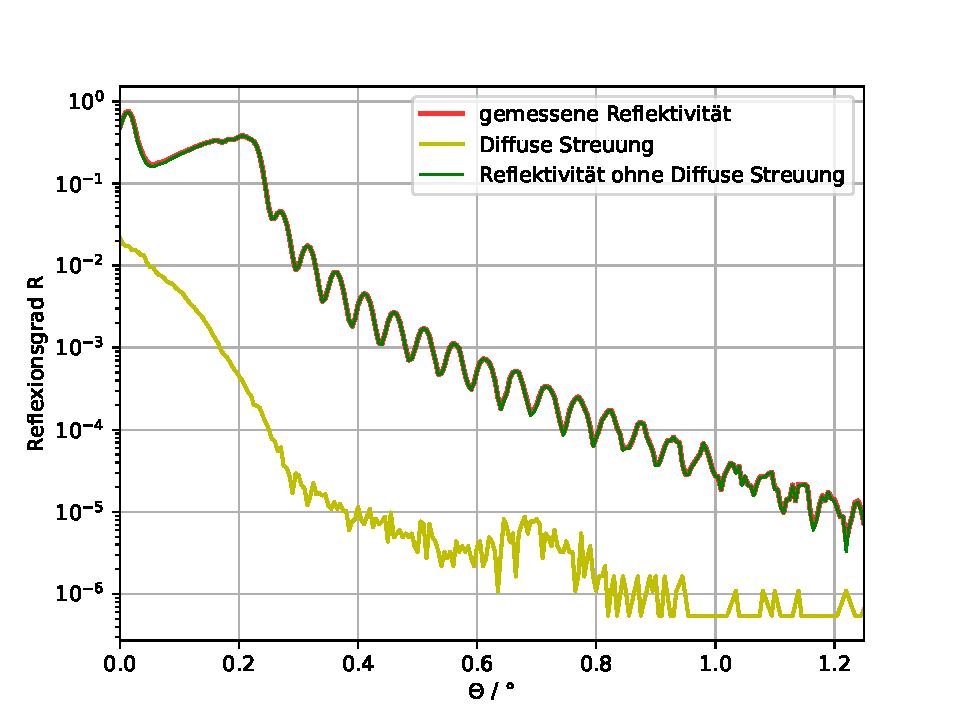
\includegraphics[width=0.8\textwidth]{plots/Reflektionsmessung.pdf}
    \caption{Reflexionsmessung in Abhängigkeit des Einfallswinkels}
    \label{fig:Reflektionsmessung}
\end{figure}

\begin{figure}[H]
    \centering
    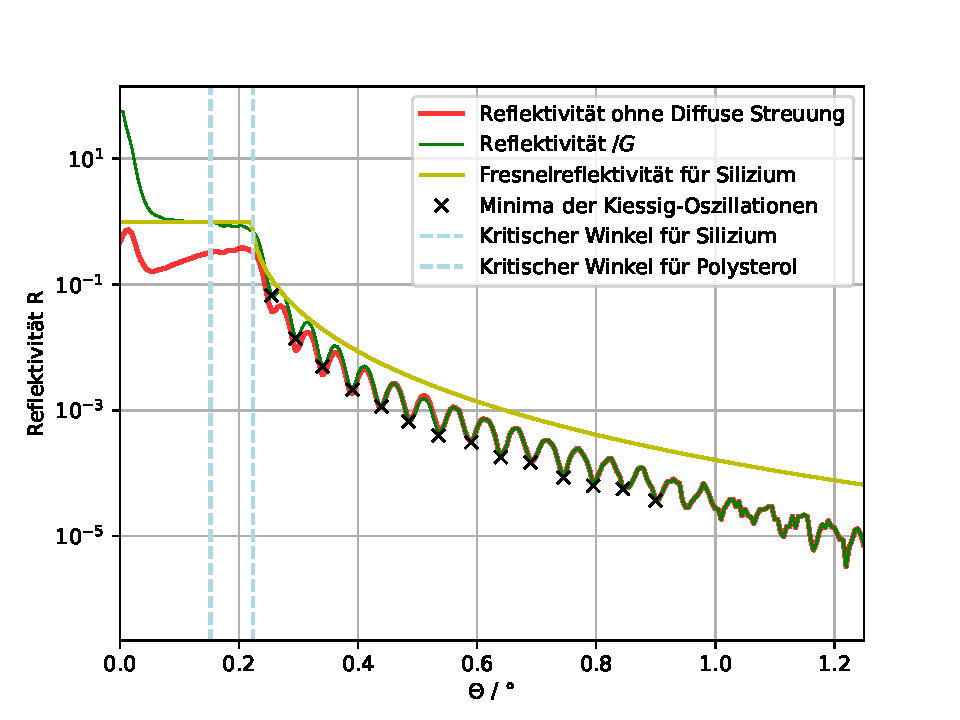
\includegraphics[width=0.8\textwidth]{plots/KorrigierteReflektionsmessung.pdf}
    \caption{Geometriefaktorkorrektur der Reflexionsmessung}
    \label{fig:KorrigierteReflektionsmessung}
\end{figure}

\begin{figure}[H]
    \centering
    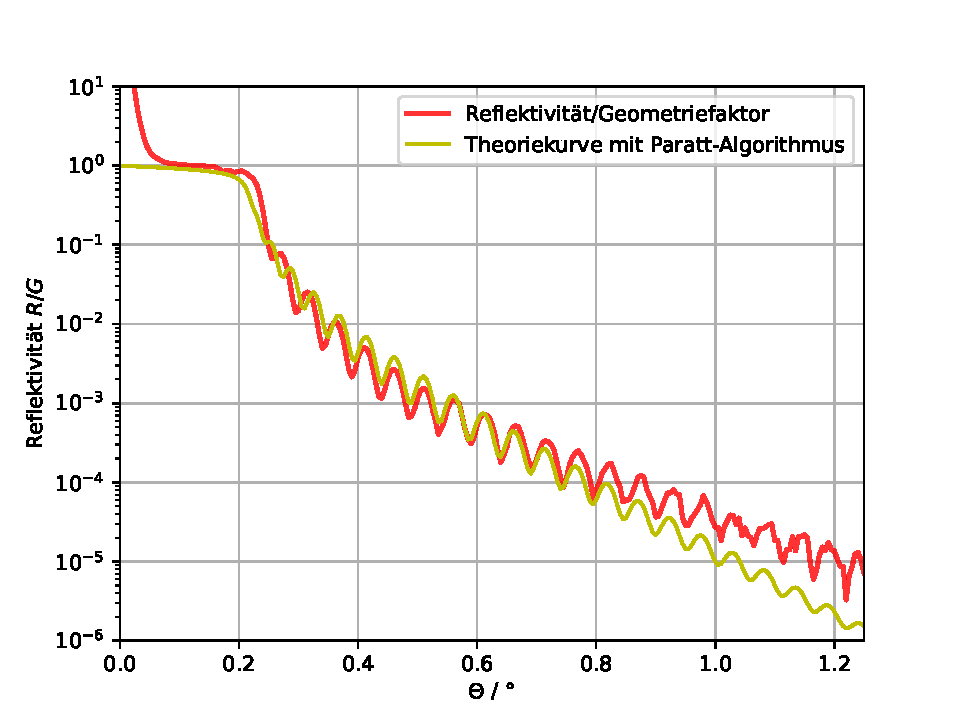
\includegraphics[width=0.8\textwidth]{plots/Parattplot.pdf}
    \caption{Näherung der Fresnelreflektivität durch das Paratt-Modell}
    \label{fig:Parattplot}
\end{figure}



